\documentclass[aspectratio=169,10pt]{beamer}

\usetheme{Madrid}
\usecolortheme{seahorse}

\definecolor{icmlblue}{RGB}{0,73,135}
\definecolor{icmlred}{RGB}{178,34,34}
\definecolor{lightgray}{RGB}{245,245,245}

\setbeamercolor{structure}{fg=icmlblue}
\setbeamercolor{title}{fg=white,bg=icmlblue}
\setbeamercolor{frametitle}{fg=icmlblue,bg=lightgray}
\setbeamercolor{block title}{fg=white,bg=icmlblue}
\setbeamercolor{block body}{fg=black,bg=lightgray}
\setbeamercolor{alerted text}{fg=icmlred}

\usepackage[utf8]{inputenc}
\usepackage{amsmath,amssymb}
\usepackage{booktabs}
\usepackage{tikz}
\usetikzlibrary{positioning,arrows.meta}

\title[OpenRouter Contract Game]{OpenRouter + Chutes:\\A Minimal Contract-Game Framing}
\author{Harvard MadSys Lab}
\institute{}
\date{\today}

\begin{document}

\begin{frame}
\titlepage
\end{frame}

\begin{frame}{1. What Is the Idea?}
\begin{columns}[T]
\begin{column}{0.55\textwidth}
\textbf{Current setup}
\begin{itemize}
    \item OpenRouter mostly buys pay-as-you-go API supply ($S_A$)
    \item This is flexible, but expensive for stable open-weight demand
\end{itemize}

\vspace{0.15cm}
\textbf{Our proposal}
\begin{itemize}
    \item Add a wholesale quota layer ($S_Q$) from a provider such as Chutes
    \item Use token-normalized credits, not a naive request quota
    \item Keep OpenRouter's external API unchanged
    \item Let routing decide which requests deserve committed credits
\end{itemize}
\end{column}

\begin{column}{0.4\textwidth}
\begin{block}{Plain-language message}
\small
We are not just selling a better router.

\vspace{0.15cm}
We are proposing a new upstream procurement primitive:
\[
\text{spot API} + \text{wholesale quota}
\]

Our routing algorithm is what makes that quota economically valuable.
\end{block}
\end{column}
\end{columns}
\end{frame}

\begin{frame}{What the Chutes Data Tells Us}
\begin{columns}[T]
\begin{column}{0.48\textwidth}
\textbf{DeepSeek-V3.1 trace on Chutes}
\begin{itemize}
    \item 13.7M real requests over 30 days
    \item Request cost is highly skewed: Gini = 0.54
    \item A small fraction of expensive requests dominates the bill
\end{itemize}

\vspace{0.15cm}
\begin{block}{Interpretation}
\small
This is exactly the setting where wholesale quota can create value:
\begin{itemize}
    \item stable enough demand to buy committed capacity
    \item enough cost skew that smart routing matters
\end{itemize}
\end{block}
\end{column}

\begin{column}{0.48\textwidth}
\centering
\begin{tabular}{lrrr}
\toprule
Quota & Smart & Greedy & Gain \\
\midrule
10\% & 38\% & 11\% & 3.6x \\
30\% & 67\% & 32\% & 2.1x \\
50\% & 83\% & 52\% & 1.6x \\
\bottomrule
\end{tabular}

\vspace{0.2cm}
\begin{alertblock}{Why this matters}
\small
Without smart routing, subscription procurement leaves a lot of value on the table.
\end{alertblock}
\end{column}
\end{columns}
\end{frame}

\begin{frame}{2. Why Is This a Game-Theory Problem?}
\begin{columns}[T]
\begin{column}{0.5\textwidth}
\textbf{Why this is not just cost accounting}
\begin{itemize}
    \item Chutes chooses whether to offer a contract $(Q,F)$
    \item OpenRouter chooses whether to accept it
    \item If accepted, OpenRouter routes requests into the covered tranche
\end{itemize}

\vspace{0.15cm}
\textbf{Minimal payoffs}
\[
\pi_{\mathrm{OR}}(Q,F;A) = V_A(Q) - F
\]
\[
\pi_{\mathrm{CH}}(Q,F;A) = F - \alpha_{\mathrm{tranche}}V_A(Q) - \Delta_K
\]
\end{column}

\begin{column}{0.44\textwidth}
\centering
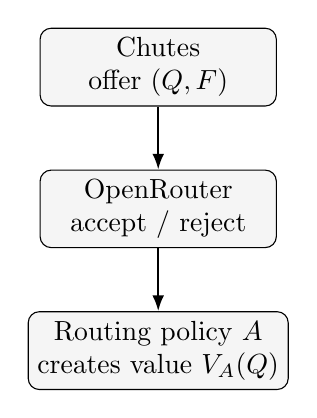
\begin{tikzpicture}[
    node distance=0.8cm and 0.8cm,
    box/.style={draw, rounded corners, align=center, minimum width=3.0cm, minimum height=0.9cm, fill=lightgray},
    arrow/.style={-{Latex[length=2mm]}, thick}
]
\node[box] (a) {Chutes\\offer $(Q,F)$};
\node[box, below=of a] (b) {OpenRouter\\accept / reject};
\node[box, below=of b] (c) {Routing policy $A$\\creates value $V_A(Q)$};
\draw[arrow] (a) -- (b);
\draw[arrow] (b) -- (c);
\end{tikzpicture}
\end{column}
\end{columns}

\vspace{0.15cm}
\begin{alertblock}{When does a win-win deal exist?}
\small
\[
(1-\alpha_{\mathrm{tranche}})V_A(Q) > \Delta_K
\]
Interpretation: the new value created by the deal must exceed the provider's extra cost.
\end{alertblock}
\end{frame}

\begin{frame}{3. Why Does Our Algorithm Matter?}
\textbf{Core point}
\begin{itemize}
    \item The contract value is not fixed
    \item Better routing captures more of the possible savings:
    \[
    V_A(Q)=\gamma_A(Q)\,V_{\mathrm{opt}}(Q)
    \]
    \item So better routing expands the feasible contract space
\end{itemize}

\vspace{0.1cm}
\centering
\begin{tabular}{lrr}
\toprule
Algorithm & Contract Zone & OR Savings \\
\midrule
Greedy & \$12,676 & 16.7\% \\
Best online (PD-EMA) & \$16,315 & 21.5\% \\
Optimal & \$22,007 & 29.1\% \\
\bottomrule
\end{tabular}

\vspace{0.15cm}
\begin{block}{What I want to confirm with the advisor}
\small
Should we present this as a bilateral contract game first, and treat auction as a later extension for the multi-provider setting?
\end{block}
\end{frame}

\end{document}
